
%\documentclass[pre,preprint,showpacs,nofootinbib]{revtex4}
\documentclass[pre,preprint]{revtex4}
%\documentclass[article]{revtex4}
\usepackage{graphicx}
\usepackage{epsfig}
%\usepackage{dcolumn}
\usepackage{amssymb,amsmath}
\usepackage{bm}
\usepackage{pdfsync}

\newcommand{\lb}{{\langle}}
\newcommand{\rb}{{\rangle}}

\begin{document}

\title{The Diameter and Other Chemical Distance of Random Clusters}

\author{Don Blair}
\author{Jon Machta}

\affiliation{Department of Physics, University of Massachusetts, Amherst, MA 01003.}
\date{\today}


% \begin{abstract}
%  A relatively unexplored geometric property of Potts models clusters is their ``diameter'', $D$ -- the longest shortest path between any two points on the cluster. We report numerical results for the fractal dimension of the diameter, $D_{min}$ and the fractal dimension of the chemical distance, $d_{min}$, for 2D critical Potts clusters with $q=1,2,3,4,5$. We find that $D_{min} = d_{min}$ within numerical error. Test. Test2. Test3.
% \end{abstract}

%\maketitle 

\section{Methods}

We used the Swendsen Wang algorithm to simulate the Potts Model with $1=1,2,3,4$ on square (dim=2) lattices of various sizes $L$, and with $q=2$ in the cubic and hypercubic lattices (dim=3,4). In the largest cluster in each of $N=10^5$ realizations, we measured the chemical distance, $l$, between two randomly chosen sites on the largest cluster, as well as the diameter $D$ of the largest cluster. For $q=1$, the standard deviation $\sigma$ in the (uncorrelated) values for $\lb l \rb$ and $\lb D \rb$ were calculated as $\sigma_{uncorr} = \sqrt{ \frac{1}{N-1} (\lb l^2 \rb - \lb l \rb^2)}$. For $q=2,3,4$, successive measurements of $l$ and $D$ were not independent; each system of size $L$ was therefore allowed to thermalize for 10*$\tau_{exp}$, where $\tau_{exp}$ is the fitted exponential correlation time for the mass of the largest cluster in the system.  The standard deviation $\sigma_{corr}$ was then considered to be $\sigma_{corr} = \sqrt{ \frac{2 \tau_{int}}{N} (\lb l^2 \rb - \lb l \rb^2)}$, where $\tau_{int}$ is the measured integrated correlation time for the chemical distance $l$.  A similar analysis was used for the diameter, $D$.


\begin{center}
\begin {table}[ht]
\addtolength{\tabcolsep}{5pt}
%\caption{Scaling exponents $d_{min}$ and $D_{min}$ for $dim=2$, $q=1,2,3,4$}
\begin{tabular}{|c| c |c|c|c|c|}
\hline
 dim  &  $q$  &  $L$                   &  $L_{min}$  &   $d_{min}$  &   $D_{min}$  \\
\hline
   2  &  1  &  16,32,48,64,96,128  &       48  &  1.131(1)  &  1.138(1)  \\
   2  &  2  &  16,32,48,64,96,128  &       48  &  1.096(1)  &  1.102(1)  \\
   2  &  3  &  16,32,48,64,96,128  &       48  &  1.065(3)  &  1.071(1)  \\
   2  &  4  &  16,32,48,64,96,128  &       48  &  1.033(3)  &  1.039(1)  \\
\hline
\end{tabular}
\caption{Scaling exponents $d_{min}$ and $D_{min}$ for $dim=2$, $q=1,2,3,4$}
\label{table:nonlin}
\end{table}
%\caption{Scaling exponents $d_{min}$ and $D_{min}$ for $dim=2$, $q=1,2,3,4$}
\end{center}


%\begin{tabular}{rrlrrl}
\begin{center}
\begin {table}[ht]
\addtolength{\tabcolsep}{5pt}
%\caption{Scaling exponents $d_{min}$ and $D_{min}$ for $dim=3,4$, $q=2$}
\begin{tabular}{|c| c |c|c|c|c|}
\hline
dim  &  $q$  &  $L$                   &  $L_{min}$  &   $d_{min}$  &   $D_{min}$  \\
\hline
   3  &  2  &  20,36,48,64,128  &       36  &  1.267(5)  &  na       \\
   4  &  2  &  12,24,36,48,64   &       24  &  1.485(7)  &  na       \\
\hline
\end{tabular}
\caption{Scaling exponents $d_{min}$ and $D_{min}$ for $dim=3,4$, $q=2$}
\label{table:nonlin}
\end{table}
\end{center}

\section{Figures}


% Figures for D=2:

% q=1, d_min

\begin{figure}[htp]
\centering
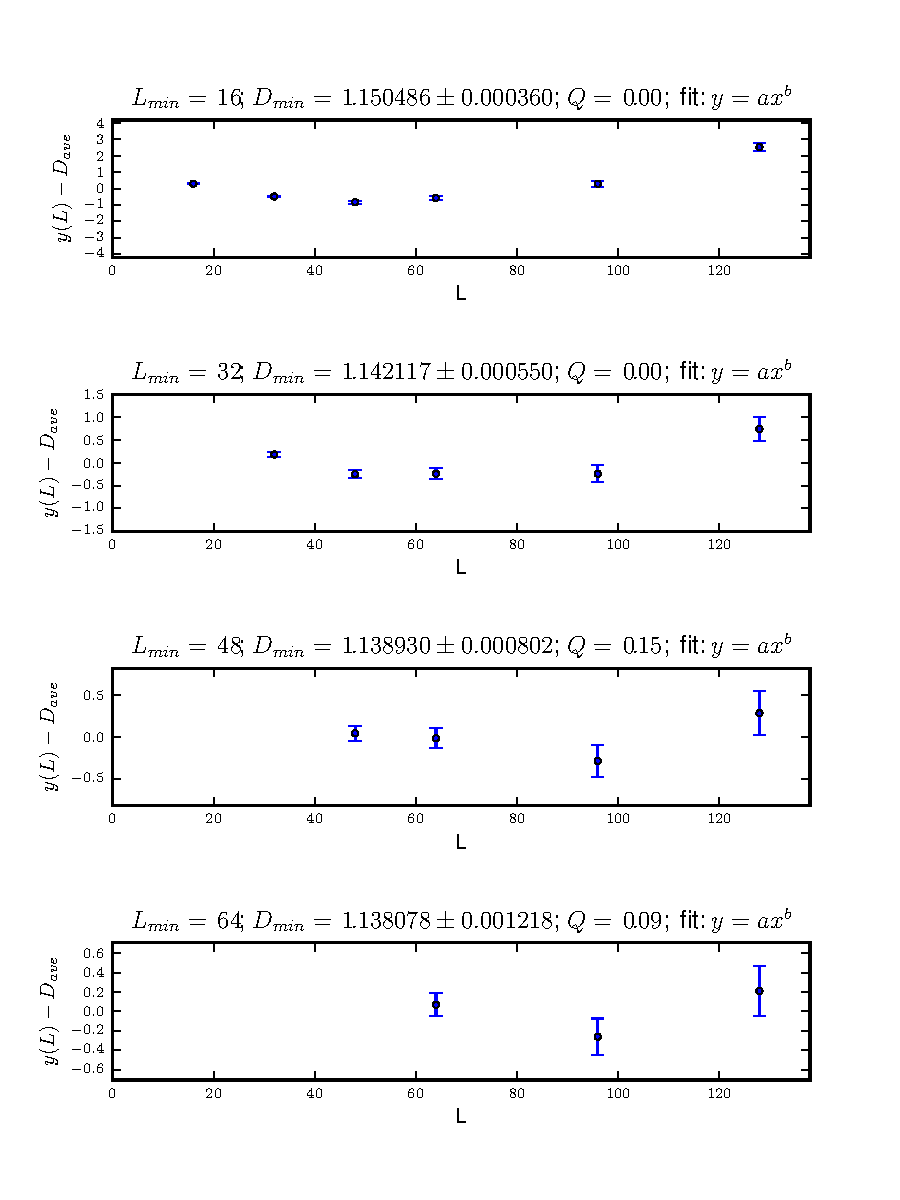
\includegraphics[width=.85\textwidth]{figures/d_min_D2q1_46_fig}
\caption{The difference between the fit, $y(L)=cL^{d_{min}}$, and the average chemical distance $\lb l \rb$ for dim=2, q=1.}\label{fig:1}
\end{figure}

%q=1, D

\begin{figure}[htp]
\centering
\includegraphics[width=.85\textwidth]{figures/D_min_D2q1_46_fig}
\caption{The difference between the fit, $y(L)=cL^{D_{min}}$, and the average diameter $\lb D \rb$ for dim=2, q=1.}\label{fig:2}
\end{figure}


%q=2, d

\begin{figure}[htp]
\centering
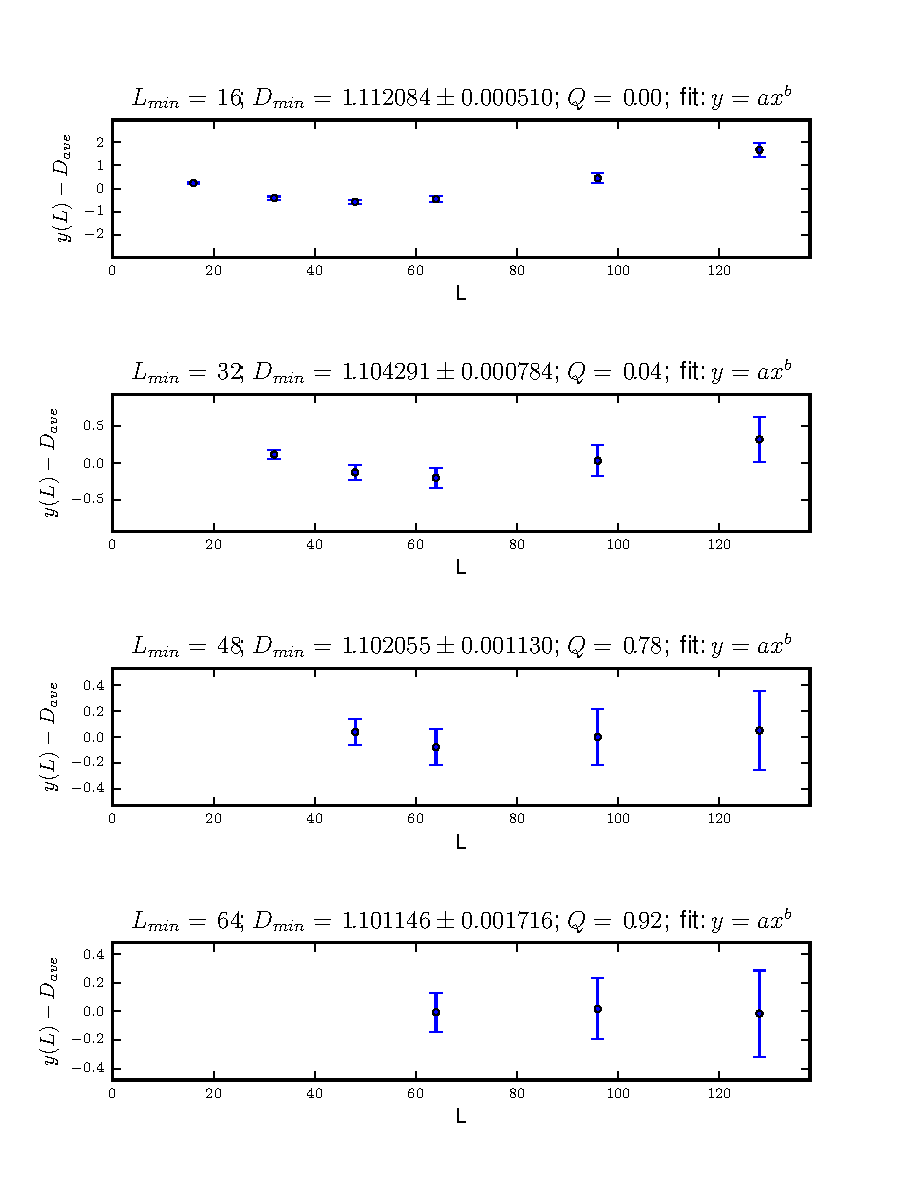
\includegraphics[width=.85\textwidth]{figures/d_min_D2q2_46_fig}
\caption{The difference between the fit, $y(L)=cL^{d_{min}}$, and the average chemical distance $\lb l \rb$ for dim=2, q=2.}\label{fig:3}
\end{figure}

%q=2, D

\begin{figure}[htp]
\centering
\includegraphics[width=.85\textwidth]{figures/D_min_D2q2_46_fig}
\caption{The difference between the fit, $y(L)=cL^{D_{min}}$, and the average diameter $\lb D \rb$ for dim=2, q=2.}\label{fig:4}
\end{figure}

%q=3, d

\begin{figure}[htp]
\centering
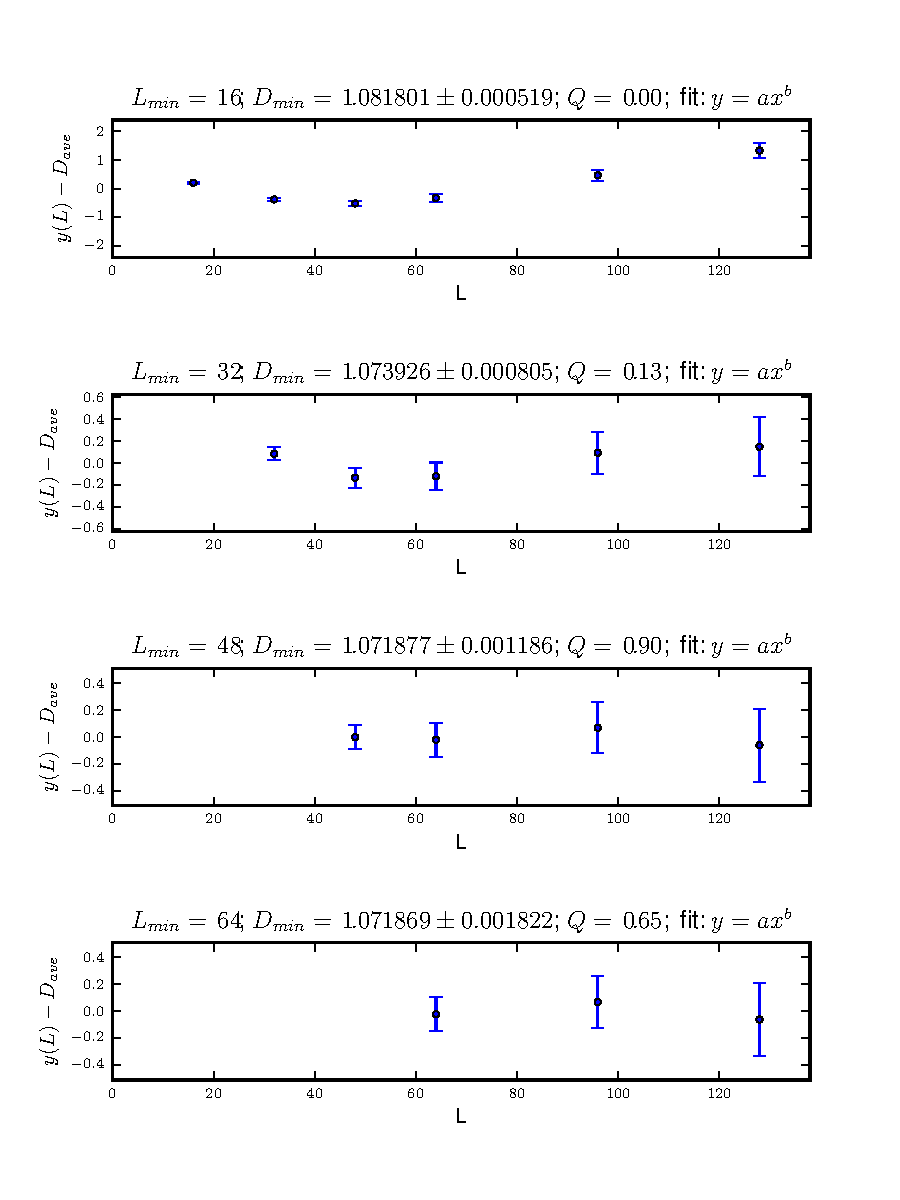
\includegraphics[width=.85\textwidth]{figures/d_min_D2q3_46_fig}
\caption{The difference between the fit, $y(L)=cL^{d_{min}}$, and the average chemical distance $\lb l \rb$ for dim=2, q=3.}\label{fig:4}
\end{figure}

%q=3, D

\begin{figure}[htp]
\centering
\includegraphics[width=.85\textwidth]{figures/D_min_D2q3_46_fig}
\caption{The difference between the fit, $y(L)=cL^{D_{min}}$, and the average diameter $\lb D \rb$ for dim=2, q=3.}\label{fig:4}
\end{figure}

%q=4, d

\begin{figure}[htp]
\centering
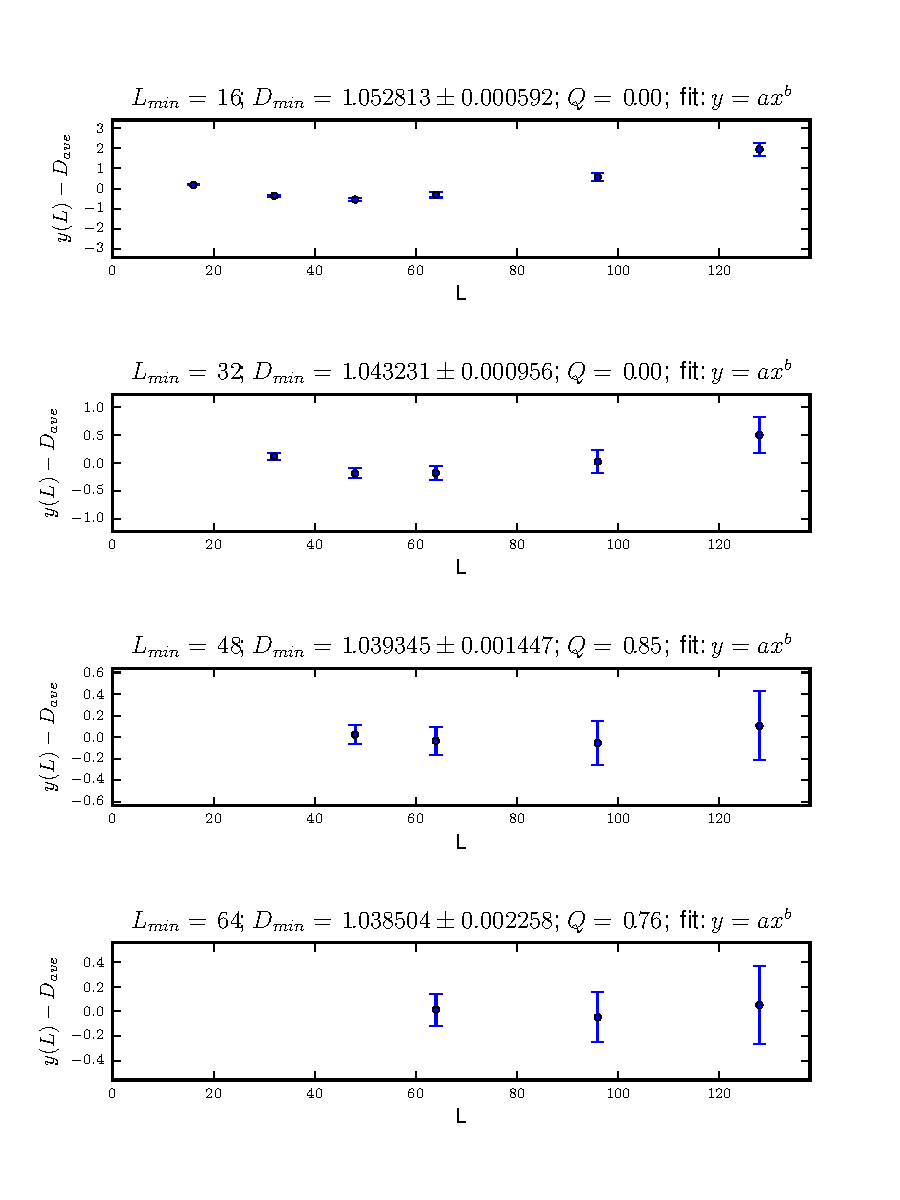
\includegraphics[width=.85\textwidth]{figures/d_min_D2q4_46_fig}
\caption{The difference between the fit, $y(L)=cL^{d_{min}}$, and the average chemical distance $\lb l \rb$ for dim=2, $q$=4.}\label{fig:4}
\end{figure}

%q=4, D

\begin{figure}[htp]
\centering
\includegraphics[width=.85\textwidth]{figures/D_min_D2q4_46_fig}
\caption{The difference between the fit, $y(L)=cL^{D_{min}}$, and the average diameter $\lb D \rb$ for dim=2, $q$=4.}\label{fig:4}
\end{figure}

%q=4, d, log fit

\begin{figure}[htp]
\centering
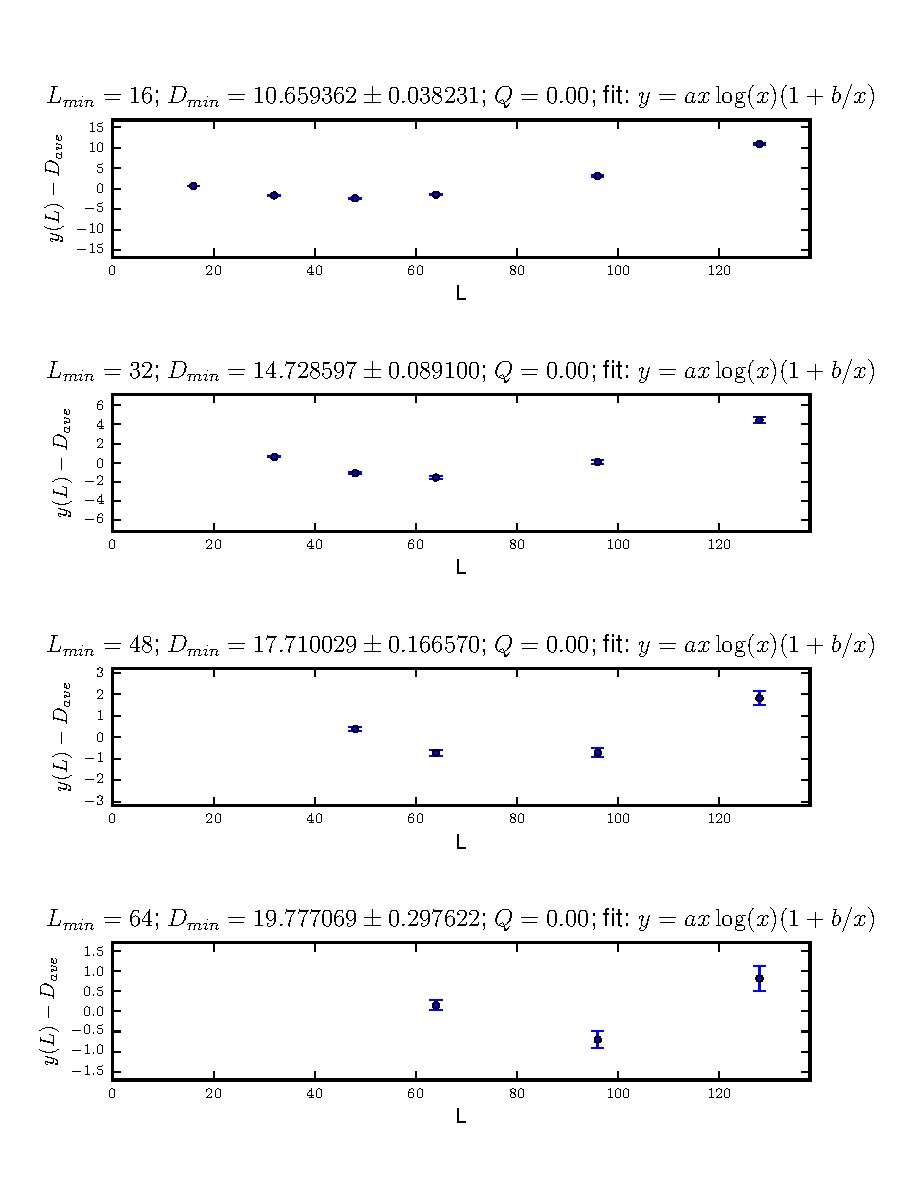
\includegraphics[width=.85\textwidth]{figures/d_min_D2q4_46_log_fig}
\caption{$d_{min}$ for D=2, q=4; log fit. Q values low -- won't use. }\label{fig:4}
\end{figure}

%q=4, D, log fit

\begin{figure}[htp]
\centering
\includegraphics[width=.9\textwidth]{figures/D_min_D2q4_46_log_fig}
\caption{$D_{min}$ for D=2, q=4; log fit. q values low -- won't use.}\label{fig:4}
\end{figure}


%D=3, q=2

\begin{figure}[htp]
\centering
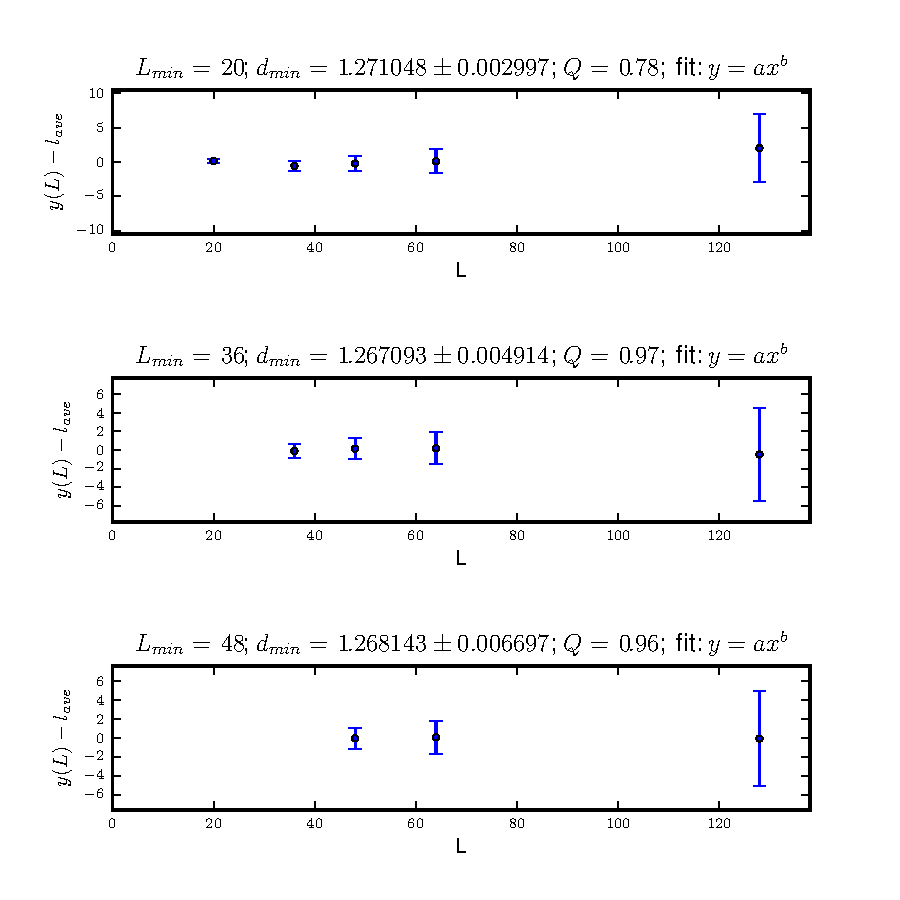
\includegraphics[width=.9\textwidth]{figures/d_min_D3q2_46_fig}
\caption{The difference between the fit, $y(L)=cL^{d_{min}}$, and the average diameter $\lb l \rb$ for dim=3, $q$=2.}\label{fig:4}
\end{figure}

%D=4, q=2

\begin{figure}[htp]
\centering
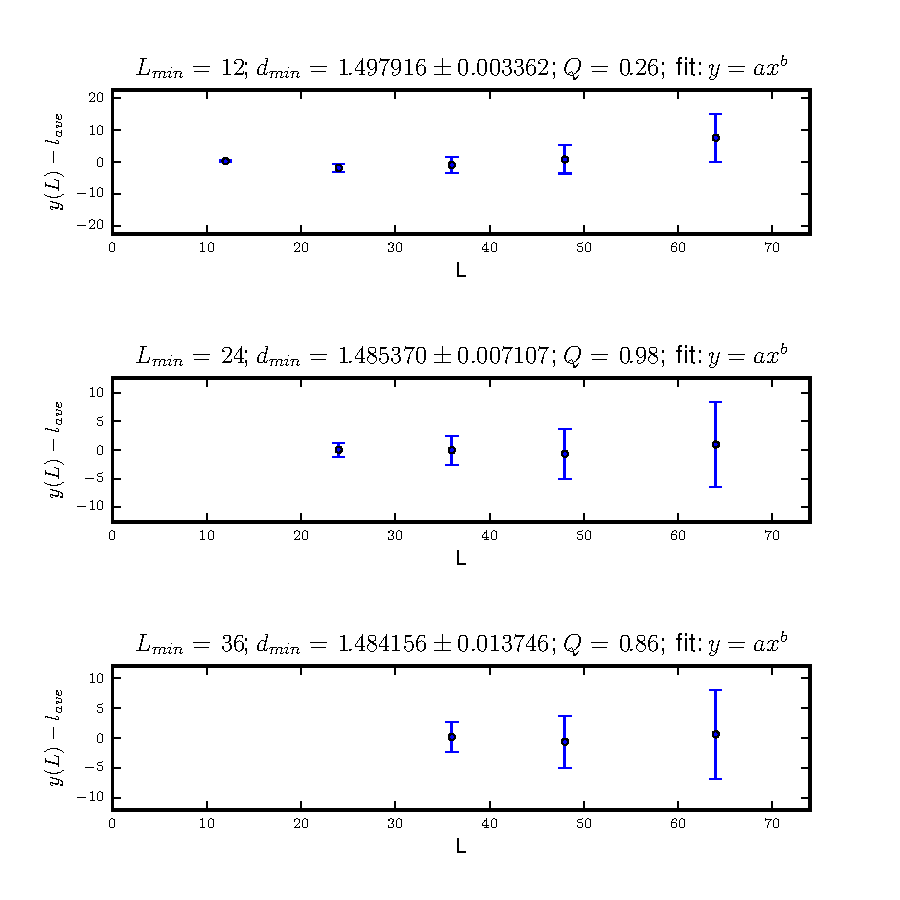
\includegraphics[width=.9\textwidth]{figures/d_min_D4q2_46_fig}
\caption{The difference between the fit, $y(L)=cL^{d_{min}}$, and the average diameter $\lb l \rb$ for dim=4, $q$=2.}\label{fig:4}
\end{figure}

\end{document}

